%----------------------------------------------------------------------------------------
%	Data Analysis Techniques
%----------------------------------------------------------------------------------------

\chapterimage{chapter_head_1.pdf} % Chapter heading image

\chapter{The Basics of Error Analysis}

There are many books on error analysis, but no physics research guide would be complete without at least an introduction to errors and experimental uncertainty. If you're interested in a more in-depth approach, some good references with exercises are:
\begin{enumerate}
\item \emph{Dealing with Uncertainties: a Guide to Error Analysis} by Manfred Drosg, 2007 -- more of a `philosophically correct' approach
\item \emph{A Student's Guide to Data and Error Analysis} by Herman J. C. Berendsen, 2011 -- a more instructive and concise approach
\item \emph{Data Reduction and Error Analysis for the Physical Sciences} by Bevington \& Robinson, 2003 -- a more encyclopedic approach
\end{enumerate}

\section{Experimental measurements and scientific results}

\begin{aquote}{-- M. Drosg (2007, pg. 1)}
``[T]here can be no scientifically relevant data without uncertainty''
\end{aquote}

The goal of error analysis is to understand exactly how accuracy and precision affect the result of an experiment, and to use this information to devise better experiments and avoid fallacious conclusions. Understanding error is essential for any physicist who wants to test the theory in the ``real world''.

In a perfectly accurate and precise experiment, there is no error analysis to speak of. Since there are no perfectly accurate or precise scientific instruments, a large part of the validity of experimental work revolves around quantifying how inaccurate and imprecise experimental observations are. 

 There is no such thing as an exact number in science \footnote{For good philosophical discussions of uncertainty in science see Karl Popper's \emph{The Logic of Scientific Discovery (2002)} or M. Drosg's  \emph{Dealing With Uncertainties (2007)}}, so it is important to know how to represent experimental results in terms of accuracy and precision.


\subsection{Accuracy and precision: stating scientific results}
The difference between accuracy and precision can be portrayed well by the statement:
\begin{quote}
{\it Accuracy is how close measurements of a physical quantity come to predicting the true value, whereas precision is how close measurements of a physical quantity are to eachother.}
\end{quote}

In an experiment, results must always be written as a value with an associated uncertainty (\emph{value $\pm$ uncertainty}). The \emph{value}, if you compare it to the accepted value or some other measurement, will give you some idea of your accuracy -- the \emph{uncertainty} will tell you your precision. One of the most important habits to get used to is quoting your error and precision in a way that makes sense. Writing $3.452673 \pm .1$  or $3.5 \pm .128619$ makes no sense -- the right number of significant digits must be used to convey to what extent you know your accuracy and your precision. Neither of these expressions works because the first ($3.452673 \pm .1$) has useless digits in the accuracy because the precision is too low and the second ($3.5 \pm .128619$) gives useless digits in the precision because the accuracy isn't high enough for the millionths place precision to be useful.

A good result has an appropriate number of significant figures in the \emph{value} and the \emph{uncertainty} that makes every digit of the result useful. When quoting uncertainty, the default is the \emph{standard deviation} or \emph{root-mean-square error} of the estimated probability distribution.  

\begin{example}
 An abstract reads ``We measure the frequency of oscillation of a comatose squirrel strapped a swingset and calculate a value of $\omega_0 = 1.34 \pm 0.07$ Hz. This is consistent with classical predictions..."

Here, the correct interpretation of $\pm 0.07$ is that it is the \emph{standard deviation} (in Hz) of a set of measured frequencies.
\end{example}

\section{Kinds of error}

In experimental, there are two basic categories of error:

\begin{enumerate}
\item { \bf Systematic Errors}: These are reproducible (but may be time dependent, watch out!) errors that cannot be reduced through statistical analysis. Common instances of this are calibration errors and false assumptions about the operation of the apparatus. These errors cannot be eliminated as there is always uncertainty in the system specificied that yields the data. 
\item { \bf Statistical Errors (Random Errors)}: These are errors that can be accounted for using statistical analysis. The typical example is a measurement which fluctuates in a gaussian or normal way about some mean. It is impossible to eliminate these errors but it is theoretically always possible to make these errors smaller than the systematic error with enough data. At some point the uncertainty as to what `identical conditions' are dominates.
\end{enumerate}

% systematic error ties to accuracy, whereas statistical error ties to precision. Not strictly but yeah intuitively in general.

Roughly speaking, systematic error has to do with accuracy and statistical error has to do with precision. Of course this is not necessarily the case: there can be nonisolatable systematic errors which yield higher uncertainties in your analysis, as well as statistical effects which 



\section{Error propagation}
\subsection{The concept of estimator}

In experiment, there is a crucial difference between the number that you calculate from some statistical formula, and the parameter you're estimating by using that formula. Because there are no exact numbers in experiment, there will necessarily be some uncertainty as to what the ``true'' value is. It is so important not to get confused between true parameters and estimates that in the following sections and in the next chapter, I denote estimates with hats $\hat{\;}$ and leave the true parameters alone. 

This is common practice in statistics, and for a proper understanding of the formulae in physics it is essential. For instance, the definition of variance $\sigma_a^2$ is that in equation \ref{variance}, but as experimenters we are limited to using an \emph{estimator} of that value ($\hat \sigma^2$) given in equation \ref{bessel}. Other authors sometimes choose $s_a^2$ to denote ``sample variance'', but I find the latin-to-greek convention there somewhat obfuscating. For every true parameter $x$ that exists in a theoretical model, I call the formula for it that uses experimental data ``$\hat x$, the estimator of $x$."

\subsection{How to estimate error in an algebraic formula}

\begin{remark}
The equations in this section are convenient for those cases in which you are either:
\begin{enumerate}
\item forced to estimate uncertainty without the use of statistics
\item sure that the uncertainty in your input is approximately the same over the range over the range of your dataset
\end{enumerate} 
\end{remark}

Whenever you have a variable which is equal to some formulation of measured variables ( an equation, for instance $P = nRT/V$), the deviation in that variable ($P$) will depend on the deviation in the other variables from their expected values. That is, if each of the variables in a formula have some uncertainty to them, the result will also have an uncertainty. Remember that in an experiment this is always true since whatever you are calculating is by definition a formulation of your measurements and all measurements have uncertainty if they are scientifically relevant. Under the assumption that the function is well-behaved (continuous and differentiable) in the region of parameters you're looking at, a simple approach to this deviation is simply to use a Taylor expansion of the formula and propagate error.

Say for instance that you have some function $f(a,b)$ of some parameters $a$ and $b$, which have errors which you expect to be about $\delta a$ and $\delta b$ large, respectively. The resulting deviation can typically be represented well by using a Taylor expansion:

\begin{equation}
|\delta f(a,b)| = \bigg | \frac{\partial f}{\partial a} \delta a \bigg | + \bigg | \frac{\partial f}{\partial b} \delta b \bigg |
\end{equation}

This equation serves as a good estimate of maximum error or deviation, but it is \emph{not} a good estimate of uncertainty. This is because the equation estimates the deviation of output based on deviation in input. Since measures of uncertainty are quoted in standard deviations and measures of statistical dispersion, an estimate of `maximum deviation' is not sufficient and will often overstate the actual error. As an example of this, consider the function $f = \alpha a + \beta b$, where $\alpha$ and $\beta$ are constants:

\begin{equation}
\delta f = \bigg | \frac{\partial f}{\partial a} \delta a \bigg | + \bigg | \frac{\partial f}{\partial b} \delta b \bigg | = |\alpha \delta a|  + |\beta \delta b|   \label{erreq}
\end{equation}

Now let's suppose that these $\delta a$ and $\delta b$ were actually fairly close to being good descriptors of standard deviation -- that is, $\sigma_a \simeq \delta a$. Assuming that the data in $a$ and $b$ were independent, the error would be:

\begin{equation}
\sigma_f = \sqrt{\bigg (  \frac{\partial f}{\partial a}\bigg )^2 \sigma_a^2 + \bigg (  \frac{\partial f}{\partial b}\bigg )^2 \sigma_b^2} = \sqrt{\alpha^2 \sigma_a^2 + \beta^2 \sigma_b^2} \label{erreq2}
\end{equation}

This is substantially different than eq. \ref{erreq}, since $\sqrt{x^2 + y^2} < x^2 + y^2$ for any two positive $x$ and $y$. In short, eq. \ref{erreq} is only a conservative bound for error which serves as a starting point in an experiment or calculation.

In summary, if you have a good estimate of the uncertainties in a function input, use \eqref{erreq} if you are in a rush and \eqref{erreq2} if you want to be thorough \emph{and} have a reason to believe the input errors should not be correlated.




\subsection{With statistical uncertainties}
Often, it is necessary to look at errors statistically. This is especially true fluctuations in the measured values vary beyond uncertainty for what are ostensibly the same experimental conditions. While it is often possible to estimate uncertainties using device specifications there is no surer method of obtaining information about random error than by repeating an experiment and getting more data.

 In the notation here, $\bar a$ denotes the mean $\sum a_i/N$, and all partial derivatives are evaluated at the mean values ($\bar a$ and $ \bar b$). It is important to keep in mind that using the statistical method of estimating uncertainties, $\sigma_f^2$ is calculated for a single point in the parameter space which we assume is ($\bar a , \bar b$)


To calculate $\sigma_f^2$, instead of using $\delta a$ we now just say that the deviations $f_i - \bar f$ are related by the same Taylor expansion to the {\it deviations in the input variables ($a_i - \bar a$ and $b_i - \bar b$) }:

\begin{equation}
f_i - \bar f \simeq \frac{\partial f}{\partial a} (a_i - \bar a) + \frac{\partial f}{\partial b} (b_i - \bar b)
\end{equation}


Since standard deviations, means, and other standard statistical results are built out of these deviations, such an expansion forms the theoretical basis for all error propagation statistics. Once a distribution of devations $f_i - \bar f$ over the data set is obtained, then we can construct $\sigma_f^2$, which is the uncertainty in our result $f$:

\begin{equation}
\sigma_f^2 = \lim_{N \to \infty}  \frac{1}{N} \sum_i ( f_i - \bar f)^2 = \lim_{N \to \infty}  \frac{1}{N} \sum_i \bigg [ \frac{\partial f}{\partial a} (a_i - \bar a) + \frac{\partial f}{\partial b} (b_i - \bar b) \bigg]^2
\label{sigmaequation1}
\end{equation}

Expanding equation \ref{sigmaequation1},

\begin{equation}
\sigma_f^2 \simeq \lim_{N \to \infty}  \frac{1}{N} \sum_i \bigg [ \bigg ( \frac{\partial f}{\partial a}\bigg )^2 (a_i - \bar a)^2 + \bigg (\frac{\partial f}{\partial b}\bigg )^2 (b_i - \bar b)^2  +  2 \bigg ( \frac{\partial f}{\partial a}\bigg )  \bigg ( \frac{\partial f}{\partial b}\bigg ) (a_i - \bar a)(b_i - \bar b) \bigg]
\label{sigmaequation2}
\end{equation}
The variance of a parameter (e.g. $a$) is:

\begin{equation}\label{variance}
\sigma_a^2 \equiv \lim_{N \to \infty}  \frac{1}{N} \sum_i (a_i - \bar a)^2 
\end{equation}

While the covariance between two statistics (e.g. $a$ and $b$) is:

\begin{equation}
\sigma_{a,b}^2 \equiv \lim_{N \to \infty}  \frac{1}{N} \sum_i (a_i - \bar a)(b_i - \bar b)
\end{equation}

This means that equation \ref{sigmaequation2} can be rewritten as
\begin{framed}
\begin{equation}\label{errprop}
\hat \sigma_f^2 = \hat  \sigma_a^2 \bigg ( \frac{\partial f}{\partial a}\bigg )^2 + \hat \sigma_b^2 \bigg ( \frac{\partial f}{\partial b}\bigg )^2  + 2 \hat \sigma_{a,b}^2\bigg ( \frac{\partial f}{\partial a}\bigg )  \bigg ( \frac{\partial f}{\partial b}\bigg )
\end{equation}
\end{framed}

This is a very important equation (often called the \emph{error propagation equation}), because it tells you how to propagate statistical error no matter your function is. Here the hats on the variances (e.g. $\hat \sigma_a^2$) denote them as {\it estimators} of the true variances (they are also sometimes called `sample variances'). It is impossible to measure an infinite number of data points, so we are limited to using \footnote{The $N-1$ in the denominator here is due to an important correction in statistics known as Bessel's correction. Without this correction the  estimator would be \emph{biased} and underestimate the true variance. Don't be surprised if no one cares about this correction, but it is the right way to do it. At $N = 10$, failing to use this correction will make these estimates of variance off by about 10\% on average}

\begin{equation}\label{bessel}
\hat \sigma_a^2 =  \frac{1}{N-1} \sum_i (a_i - \bar a)^2, \; \; \; \; \; \; \hat \sigma_{a,b}^2  = \frac{1}{N-1} \sum_i (a_i - \bar a)(b_i - \bar b)
\end{equation}

Some common examples of error propagation for different functions of $x$ and $y$ ($c$ and $d$ are constants):

\begin{table}
 \centering
\begin{tabularx}{250pt}{|c|X|c|X|}
  \hline 
    Function & Propagation \\ \hline    \hline
    $f = cx + dy$ 	& 	$\hat \sigma_f = \sqrt{c^2 \hat \sigma_x^2 +d^2 \hat \sigma_y^2}$    	\vspace{2 mm}\\ \hline
    $f = cx - dy$ 	& 	$\hat \sigma_f = \sqrt{c^2 \hat \sigma_x^2 +d^2 \hat \sigma_y^2}$ 	\vspace{2 mm}\\ \hline
    $f = cxy $			&  $\hat \sigma_f = c\sqrt{\bar y^2\hat  \sigma_x^2+\bar x^2 \hat \sigma_x^2}$		\vspace{2 mm}\\ \hline
    $f = cx/y $		&  $\hat \sigma_f = \frac{c}{\bar y}\sqrt{\hat \sigma_x^2 + \frac{1}{\bar y}\hat \sigma_y^2}$	\vspace{2 mm}	\\ \hline 
    $f = ce^{-dx}$ &  $\hat \sigma_f = cde^{-d\bar x}\hat \sigma_x$	\vspace{2 mm}	\\ \hline
\end{tabularx}
\end{table}


To actually make this calculation, many programs have the ability to calculate what is called a covariance matrix. This is the matrix:

\[ \Sigma = \left[ \begin{array}{cccc}
\hat \sigma_{11}^2 & \hat \sigma_{12}^2 & \ldots & \hat \sigma_{1m}^2 \\
\hat \sigma_{21}^2 & \hat \sigma_{22}^2 & \ldots & \hat \sigma_{2m}^2 \\
\vdots & \vdots & \ddots & \vdots \\
\hat \sigma_{m1}^2 & \hat \sigma_{m2}^2 & \ldots & \hat \sigma_{mm}^2 \end{array} \right].\]

Most of the time, this matrix will be essentially diagonal since the variables you will be looking at will be independent. Sometimes though, these off-diagonal terms will be indicative of some physics you haven't taken into account (e.g. temperature fluctuations).

\begin{example}
Let's say that $\ell$ and $\kappa$ are constants and you are calculating resistance across two elements in series using the following formula:
\begin{equation}
R = \ell \frac{V_1}{I_1} + \kappa \frac{V_2}{I_2}
\end{equation}
To estimate the uncertainty in $R$ at that point, one would first calculate the error propagation for the equation. To do this we find the partial derivatives:

\begin{align*}
	\frac{\partial R}{\partial V_1} &= \frac{\ell}{I_1} 		&	\frac{\partial R}{\partial I_1} = -\ell \frac{V_1}{I_1^2} 	\\
  	\frac{\partial R}{\partial V_1} &= \frac{\kappa}{I_2}  	&	\frac{\partial R}{\partial I_1} = -\kappa \frac{V_2}{I_2^2}
\end{align*}

and insert them into the error progation equation:

\begin{align*}
\sigma_R^2 \simeq   \; & \sigma_{V_1}^2 \bigg ( \frac{\partial R}{\partial V_1}\bigg )^2 + \sigma_{I_1}^2 \bigg ( \frac{\partial R}{\partial I_1}\bigg )^2  + \sigma_{V_2}^2 \bigg ( \frac{\partial R}{\partial V_2}\bigg )^2 + \sigma_{I_2}^2 \bigg ( \frac{\partial R}{\partial I_2}\bigg )^2   \\ &+ 2\sigma_{V_1,I_1}^2\bigg ( \frac{\partial R}{\partial V_1}\bigg )  \bigg ( \frac{\partial R}{\partial I_1}\bigg )  + 2\sigma_{V_2,I_1}^2\bigg ( \frac{\partial R}{\partial V_1}\bigg )  \bigg ( \frac{\partial R}{\partial I_1}\bigg ) + 2\sigma_{V_1,I_1}^2\bigg ( \frac{\partial R}{\partial V_1}\bigg )  \bigg ( \frac{\partial R}{\partial I_1}\bigg ) + 2\sigma_{V_1,I_1}^2\bigg ( \frac{\partial R}{\partial V_1}\bigg )  \bigg ( \frac{\partial R}{\partial I_1}\bigg ) \\ &  + 2\sigma_{V_1,V_2}^2\bigg ( \frac{\partial R}{\partial V_1}\bigg )  \bigg ( \frac{\partial R}{\partial V_2}\bigg )  + 2\sigma_{I_1,I_2}^2\bigg ( \frac{\partial R}{\partial I_1}\bigg )  \bigg ( \frac{\partial R}{\partial I_2}\bigg )
\end{align*}

This is a very large formula, but there are ways to calculate this faster using a computer.
If you have made $n$ measurements of the state vector $(V_1, I_1, V_2, I_2)$ at the same experiment settings, then you should have your data in an $n \times 4$ matrix. If you're using MATLAB and you've named your data matrix \texttt{data}, the command to get this covariance matrix is simply \texttt{cov(data)}. In Mathematica, the command is similar: \texttt{Covariance[data]}. Though the equation that propagates the error may be huge, it can be easy to calculate all at once if you're clever about how you use your matrices.

\end{example}


%%%
%----------------------------------------------------------------------------------------
%	Data Analysis Techniques
%----------------------------------------------------------------------------------------

\chapterimage{chapter_head_1.pdf} % Chapter heading image

\chapter{Fitting models to data}

\section{Curve-fitting concepts}

At the heart of all curve-fitting and regression techniques is an optimization problem:
\begin{quote}
\emph{Given a set of data with the associated uncertainties and a set of assumptions about the physics of the system, what is the best mathematical model that describes the data?}
\end{quote}
The issue with this kind of statement is understanding what ``best model'' means. It is important to recognize that while a model may fit the experimental data very well, it might not be very scientifically descriptive. There are two extremes in analysis that the physicist must get used to avoiding:
\begin{enumerate}
\item {\it Overcomplicating:} Because of the way the math works, it is always possible to find a model complex enough to account for all the data. For example, you could always find a fourier series or a polynomial expansion which fits every point in the dataset. This is a big mistake because the goal is not to fit the data with ad hoc assumptions that look nice but to explain the data well using physical theories and principles.
\item {\it Oversimplifying:} It is easy to be afraid of overcomplicating the problem and go too far in the other direction by ignoring other physical processes and opting for simple descriptions that don't use the data to their fullest potential. For example, you might be tempted cut out half of your data because they are noisy or don't fit well. This should be treated with caution since all errors are explainable and may be indicative of different physics.
\end{enumerate}
A good maxim to live by is ``Everything should be made as simple as possible but no simpler'' (attributed to Einstein, but he only said something similar). The model you use should be justified by the physics of the experiment. It is OK to model the things you don't know much about, but this is always dangerous territory and it is important to proceed with caution.
\section{The basics of linear least squares fitting}
In the foundations of scientific analysis some conventions have emerged that are handy both practically and theoretically. For instance, one definition of ``best'' developed by Gauss in the 19th century is that of the least squares criterion. This is the statement that under usual conditions (Gauss-Markov conditions) the best fit of a linear model to data will be the one that minimizes the sum of squared errors. The main Gauss-Markov conditions (assumptions) that guarantee this mathematically can be summarized below:
\begin{enumerate}
\item The situation the model describes actually is linear. If it's not then more complicated work may be required (e.g. nonlinear least squares).
\item The random error averages to zero -- the noise in the signal does not push the data in any particular direction \emph{on average}.
\item The error or noise in the data is about the same size over the whole dataset. When this is not true the data are said to be \emph{heteroskedastic} and the model needs to be adjusted to focus on the more precise data.
\item The noise in the data is independently distributed throughout the dataset. This means that for two data points, no amount of information about one error can tell me anything about the other.
\end{enumerate}

Even when these conditions aren't strictly true, least-squares algorithms usually do very well, especially in physics where the data are often very consistent and noise isn't that bad.
\begin{example} Let's say you measure a voltage and it fluctuates around some value in some gaussian way:

\begin{equation}
V_i = V_0 + \epsilon_i , \; \; \; \; \; \epsilon_i \sim N(\mu, \sigma_\epsilon^2) \label{meanv}
\end{equation}

The equation above says that every measured voltage $V_i$ is equal to some nominal voltage $V_0$ with some gaussian noise term $\epsilon_i$. Since we can never know $V_0$ with absolute certainty, we must come up with an estimator for it. According to the least-squares logic this will be the $\hat V_0$ that minimizes the quantity $SSR$ (the sum of squared residuals):
\begin{equation}
SSR = \sum_i \hat\epsilon_i^2 = \sum_i (V_i - \hat V_0)^2
\end{equation}
Note that $\hat \epsilon_i$ is the estimator for $\epsilon_i$ expressed as $\hat \epsilon_i = V_i - \hat V_0$. To find the optimal $\hat V_0$, just solve the first order conditions:

\begin{equation}
\frac{\partial SSR}{\partial \hat V_0} = 0 =  \sum_i -2(V_i - \hat V_0) \implies \hat V_0 = \frac{1}{N} \sum_i^N V_i 
\end{equation}
Which is the same as the mean of the voltage data. This confirms something we have been using all our lives -- under the right conditions \emph{the sample mean is a good estimate of the true mean}.
\end{example}

\section{The linear fit (Part I): OLS regression with one dependent variable}
The most typical example of an ordinary least squares (OLS) linear regression is that of the form:
\begin{equation}
y_i = \alpha + \beta x_i + \epsilon_i
\end{equation}
since it is the next simplest linear equation after \eqref{meanv}.

\subsection{Finding fit parameters}
To find estimators $\hat \alpha$ and $\hat \beta$ of the true parameters $\alpha$ and $\beta$, we first find the sum of squared errors:

\begin{equation}
SSR = \sum_i (y_i - \hat \alpha - \hat \beta x_i)^2
\end{equation}

and then solve the first order conditions:

\begin{align}
\frac{\partial SSR}{\partial \hat \alpha} = 0 &= \sum_i -2(y_i - \hat \alpha - \hat \beta x_i) & \frac{\partial SSR}{\partial \hat \beta} =0 =  \sum_i -2x_i (y_i - \hat \alpha - \hat \beta x_i) 
\end{align}
This gives us two equations with two unknowns. If the formula were more complicated and had $n$ unknowns, there would be $n$ equations from first order conditions. For a linear fit like this there is \emph{always} an analytic expression for the parameters that minimize the $SSR$. From the first equation we find that $\hat \alpha = \bar y - \hat \beta \bar x$. Substituting to find $\hat \beta$ we find:

\begin{align*}
0 &=  \sum_i x_i (y_i - \bar y + \hat \beta \bar x - \hat \beta x_i) \\
0 &=  \sum_i x_i y_i - x_i \bar y +\hat \beta \bar xx_i - \hat \beta x_i^2 \\
\hat \beta \sum_i   x_i^2 - \bar xx_i  &= \sum_i x_i y_i - x_i \bar y \\
\hat \beta &= \frac{\sum_i x_i y_i - \bar x \bar y}{\sum_i   x_i^2 - \bar x^2}
\end{align*}
This is how a least-squares algorithm will calculate the best fit:
\begin{framed}
\begin{align}
\hat \beta &= \frac{\sum_i x_i y_i - \bar x \bar y}{\sum_i   x_i^2 - \bar x^2} = \frac{\mathrm{Cov(x,y)}}{\mathrm{Var(x)}} = \frac{\langle xy\rangle-  \langle x \rangle\langle y \rangle}{\langle x^2\rangle-  \langle x \rangle^2}     & \hat \alpha =& \bar y - \hat \beta \bar x = \langle y \rangle - \langle x \rangle \bigg [\frac{\langle xy\rangle-  \langle x \rangle\langle y \rangle}{\langle x^2\rangle-  \langle x \rangle^2} \bigg]
\end{align}
\end{framed}

\subsection{Finding uncertainties in fit parameters}
At this point it is useful to look back at the sum of squared residuals:
\begin{equation}
\hat \sigma_\epsilon^2 = \frac{1}{N-k}\sum_i \hat \epsilon_i^2 =  \frac{1}{N-2}\sum_i (y_i - \hat y)^2  
\end{equation}
where the $N-k$ represents the number of \emph{degrees of freedom} ($k$ is the number of parameters). In this case there are $N-2$ degrees of freedom, since if we knew $N-2$ of the residuals, we could solve for the remaining two using the first-order conditions on $\hat \alpha$ and $\hat \beta$. This estimate is useful in finding the \emph{standard error of the regression} or \emph{root mean squared error} given by:
\begin{equation}
\hat \sigma_\epsilon = \sqrt{\hat \sigma_\epsilon^2} = \sqrt{ \frac{1}{N-2}\sum_i (y_i - \hat y)^2 }
\end{equation}
The standard deviation of  $\hat \beta$ can then be found as  $\hat \sigma_\epsilon / \mathrm{Var}(x)$. To see this, let's look at $\hat \beta$ again, substituting in $y_i = \alpha + \beta x_i + \epsilon_i$ and $\bar y = \alpha + \beta \bar x + \bar \epsilon$:
\begin{equation}
\hat \beta = \frac{\sum_i x_i y_i - \bar x \bar y}{\sum_i   x_i^2 - \bar x^2} = \frac{\sum_i x_i (\alpha + \beta x_i + \epsilon_i) - \bar x ( \alpha + \beta \bar x + \bar \epsilon)}{\sum_i   x_i^2 - \bar x^2} 
\end{equation}
which simplifies to:
\begin{equation}
\hat \beta = \beta + \frac{\sum_i x_i \epsilon_i - \bar x \bar \epsilon}{\sum_i   x_i^2 - \bar x^2}  = \beta + \frac{\mathrm{Cov}(x,\epsilon)}{\mathrm{Var}(x)}
\end{equation}
Ideally, the noise $\epsilon_i$ isn't correlated with $x_i$ so that on average $\mathrm{Cov}(x,\epsilon) = 0$.  In every dataset, no matter how large, the sample covariance will not be zero and $\hat \beta \neq \beta$. Since it \emph{approaches} zero in the limit of large numbers, more data imply a better measure of $\hat \beta$. It is important to remember that $\beta$ itself is \emph{not} random, but that only the estimator $\hat \beta$ is distributed due the random error $\epsilon_i$. At this point we are able to use the familiar error propagation equation (eq. \eqref{errprop}) to find the standard deviation of our estimator ($\epsilon_i$ and $\epsilon_j$ are independent):
\begin{equation}
\sigma_{\hat \beta} = \sqrt{\sum_i \bigg( \frac{\partial \hat \beta}{\partial \epsilon_i} \bigg )^2 \sigma_{\epsilon_i}^2}
\end{equation}

To do this we must obtain the partial derivative:
\begin{equation}
\frac{\partial \hat \beta}{\partial \epsilon_i} = 0 + \frac{\partial}{\partial \epsilon_i}  \frac{\sum_i x_i \epsilon_i - \bar x \bar \epsilon}{\sum_i   x_i^2 - \bar x^2} = \frac{\partial}{\partial \epsilon_i}  \frac{\sum_i \epsilon_i (x_i - \bar x)}{\sum_i   x_i^2 - \bar x^2} = \frac{x_i - \bar x}{\sum_i   x_i^2 - \bar x^2}
\end{equation}
Of course, in the sum \emph{this} is where the facts that the error is identically distributed and that $\epsilon_i$ and $\epsilon_j$ are independent become very important:
\begin{align}
\sigma_{\hat \beta} &= \sqrt{\sigma_{\epsilon}^2  \frac{ \sum_i (x_i - \bar x)^2}{(\sum_i   x_i^2 - \bar x^2)^2} } = \frac{\sigma_{\epsilon}}{\sum_i  ( x_i^2 - \bar x^2)}\sqrt{ \sum_i (x_i - \bar x)^2}\\
&= \frac{\sigma_{\epsilon_i}}{\sqrt{\sum_i  ( x_i^2 - \bar x^2)}}
\end{align}

Again, we can never know $\sigma_\epsilon$ exactly. The best we can do is estimate (use the estimator $\hat \sigma_\epsilon$):
\begin{framed}
The uncertainty in $\sigma_{\hat \beta}$ is therefore:
\begin{equation}
\hat \sigma_{\hat \beta} = \frac{\hat \sigma_{\hat \epsilon_i}}{\sqrt{\sum_i  ( x_i^2 - \bar x^2)}} = \frac{\sqrt{ \frac{1}{N-2}\sum_i (y_i - \hat y)^2 }}{\sqrt{\sum_i  ( x_i^2 - \bar x^2)}}
\end{equation}
The uncertainty in $\hat \alpha$ can then be found by propagating the error in $\hat \alpha = \bar y - \hat \beta \bar x$:
\begin{equation}
\hat\sigma_{\hat \alpha} = \sqrt{\bigg ( \frac{\partial \hat \alpha}{\partial \hat \beta}\bigg )^2 \sigma_{\hat \beta}^2} = \bar x \hat \sigma_{\hat \beta}
\end{equation}
\end{framed}

\section{The linear fit (Part II): using error bars in a linear fit (WLS or $\chi^2$ regression)}

So far, in using the least-squares method we've treated all datapoints as if they were of equal importance. When you do an experiment and know some of the data points to higher precision than others, there is a way to incorporate this into the analysis using something called weighted least squares regression (WLS regression). Mathematically, this is the same as saying that at $x_i$ the error $\epsilon_i$  has a true standard deviation $\sigma_i$, but at $x_j$ the error $\epsilon_j$ has a true standard deviation of $\sigma_j$ where $\sigma_i \neq \sigma_j$. Now it isn't true that the $\epsilon_i$ are identically distributed. \emph{When the error term is not identically distributed (your error bars aren't all the same size -- i.e. heteroskedasticity), the OLS estimators will be {\bf unbiased} but they {\bf will not be minimum variance. That means that if you use the method in the last section, your estimates for the parameters $\alpha$ and $\beta$ will be as accurate but less precise on average.}}

To correct for this problem, instead of minimizing the sum of squared residuals ($SSR$), we instead minimize a quantity called $\chi^2$;
\begin{equation}
\chi^2(\hat \alpha, \hat \beta) = \sum_i \bigg (\frac{y_i - \hat y_i}{\hat \sigma_i} \bigg )^2= \sum_i \bigg (\frac{y_i - (\hat \alpha + \hat \beta x_i)}{\hat \sigma_i}\bigg )^2
\end{equation}
Here, the $\hat \sigma_i$ are the values of uncertainty calculated from the characteristics of the apparatus (the error bars). This is the same as saying that the data points with low uncertainty $\hat \sigma_i$  (higher precision) are weighted more highly in the fit than those with higher uncertainty (in a specific way). When the error $\epsilon_i$ is corrected by $\sigma_i$, the error $\epsilon_i^* = \epsilon_i/\sigma_i$ is identically distributed and the problem is the same as before. 
%If we transform our model by dividing by $\sigma_i$ ($y_i \to y^*_i = y_i/\sigma_i$, $y_i \to x^*_i = x_i/\sigma_i$, and $\epsilon_i \to \epsilon^*_i = \epsilon_i/\sigma_i$), we return to a format which is more familiar:
%
%\begin{equation}
%\frac{y_i}{\sigma_i} = \alpha + \beta \frac{x_i}{\sigma_i} + \frac{\epsilon_i}{\sigma_i} \Longleftrightarrow y^*_i = \alpha + \beta x^*_i + \epsilon^*_i
%\end{equation}

In the last section we went manually through the calculation to find the parameters $\hat \alpha$ and $\hat \beta$. In this section we'll use matrices which can make solving this problem a little bit easier on the computer. WLS regression is exactly like OLS regression except each of the points is weighted.
\subsection{Matrices help to make solving fits faster (especially WLS)}
Again, as before, minimizing $\chi^2$ is like minimizing $SSR$ only the equation looks beefier since we have weighted the terms according to their precision:

\begin{align}
\frac{\partial \chi^2}{\partial \hat \alpha} = 0 &= \sum_i \frac{-2(y_i - \hat \alpha - \hat \beta x_i)}{\hat \sigma_i^2} & \frac{\partial \chi^2}{\partial \hat \beta} =0 =  \sum_i \frac{-2x_i (y_i - \hat \alpha - \hat \beta x_i) }{\hat \sigma_i^2}
\end{align}
This leaves us with two equations and two unknowns (again) :
\begin{align}
\sum_i \frac{y_i}{\hat \sigma_i^2} &= \hat \alpha \sum_i \frac{1}{\hat \sigma_i^2} + \hat \beta \sum_i \frac{x_i}{\hat \sigma_i^2}       & \sum_i \frac{x_iy_i}{\hat \sigma_i^2} &= \hat \alpha \sum_i \frac{x_i}{\hat \sigma_i^2} + \hat \beta \sum_i \frac{x_i^2}{\hat \sigma_i^2}  
\end{align}

This can be put into a matrix equation as:
\begin{equation}
\underbrace{\begin{bmatrix}
  \sum_i \frac{y_i}{\hat \sigma_i^2} \\
  \sum_i \frac{x_iy_i}{\hat \sigma_i^2} \\
 \end{bmatrix}}_{\vec c}
=
\underbrace{\begin{bmatrix}
 \sum_i \frac{1}{\hat \sigma_i^2} & \sum_i \frac{x_i}{\hat \sigma_i^2} \\
 \sum_i \frac{x_i}{\hat \sigma_i^2} &  \sum_i \frac{x_i^2}{\hat \sigma_i^2}   \\
 \end{bmatrix}}_{A}
\underbrace{\begin{bmatrix}
\hat \alpha \\
\hat \beta
 \end{bmatrix}}_{\vec m}
\end{equation}

This matrix is in the form of $A\vec m = \vec c$. Here, $\vec m$ denotes the vector of model parameters , and the vector $\vec c$ and matrix $A$ represent constraints derived from first order conditions,. It is extremely unlikely that the matrix $A$ will not be invertible, so the solution is simply $A^{-1} \vec c = \vec m$. Creating these vectors and matrices may seem simple, but a \emph{really} fast way of getting these matrices is to use a matrix representing the data used in the regression:

\begin{align}
X_{OLS} &= \begin{bmatrix}
  1 & x_1 \\
  1 & x_2 \\ 
  \vdots & \vdots \\
 1 & x_n
 \end{bmatrix}
 &X_{WLS} = \vec w \odot X_{OLS} = \begin{bmatrix}
1/\sigma_1 & x_1/\sigma_1 \\
  1/\sigma_2 & x_2/\sigma_2 \\ 
  \vdots & \vdots \\
 1/\sigma_n & x_n/\sigma_n
 \end{bmatrix}
\end{align}

Here $\odot$ represents element-wise multiplication. In MATLAB for instance, multiplying vectors or matrices (\texttt{A} and \texttt{B}) can be done element-wise with the command \texttt{A.*B}. When you use these matrices, it is very easy to construct $\vec c$ and $\vec A$:

\begin{align}
\vec c &= X^\intercal \vec y &A =  X^\intercal X
\end{align}


In summary, $\chi^2$ or WLS fitting uses exactly the same mathematics as OLS fitting, except that weighting each point makes calculating fit parameters and uncertainties involve more operations. { \bf In general, you should use the  $\chi^2$ method of least-squares fitting because it is almost always true that the error bars you use are not all the same size. If they are, it turns out that the $\chi^2$ method will give you the same result as the OLS method.} This is actually very easily provable:

\begin{equation}
\hat \sigma_i = \hat \sigma \forall i \implies \chi^2 = \sum_i  \frac{(y_i - \hat y_i)^2}{\hat \sigma_i^2} = \frac{1}{\hat \sigma^2} \sum_i (y_i - \hat y_i)^2 = \frac{SSR}{\hat \sigma^2} 
\end{equation}
Since $\hat \sigma_i$ is the same size throughout the dataset, it can be factored out of the sum, yielding the sum of squared residuals, the function to be minimized in OLS fitting. Dividing the $SSR$ by a constant does not change where the minimum is located, so the parameters you solve for must be the same.

\subsection{Uncertainties in $\chi^2$ fitting}

The uncertainty in fit parameters can be found in the $\chi^2$ fitting the same way as in the OLS case: that is, we must propagate error. In the interest of brevity, the derivation will not be shown here. Using matrices, a pattern emerges which is quite convenient (which you can derive if you want).  As it turns out, the matrix we already calculated from first-order conditions ($A^{-1}$) contains all the information necessary to propagate error.

The model parameters are given in order in a vector by  $\vec m = A^{-1}\vec c =  (X^\intercal X)^{-1} X^\intercal \vec y$. With the residuals defined as the difference between the data and the model ($\vec \epsilon = \vec y - X \vec m $), the uncertainty in each parameter is obtained as:

\begin{align}
\hat \sigma_{i} &= \hat \sigma_\epsilon \sqrt{ (A^{-1})_{i,i}} \; \; &\mbox{where}\; \;  &\hat \sigma_\epsilon^2 = \sum_i \frac{\hat \epsilon^2}{N-k} = \sum_i \frac{(y_i - \hat y_i)^2}{N-k}
\end{align}

Here the $\hat \sigma_i$ is the estimated uncertainty in the $i$-th parameter ($\hat \sigma_\alpha = \hat \sigma_1$ and $\hat \sigma_\beta = \hat \sigma_2$), the element $(A^{-1})_{i,i}$ is the $i$-th element on the diagonal of the matrix $A^{-1}$.


\section{Nonlinear fitting}

When you fit a curve to data -- no matter how many linear variables you put in the formula -- there is an analytic expression for the fit parameters that minimizes the sum of squared errors (sum of squared residuals $SSR$ or $\chi^2$ in the weighted case). This must always be true, since when you have linear combinations of parameters, the first-order conditions must generate a set of $n$ equations with $n$ unknowns. 

However, when you have a \emph{nonlinear} model, the first-order condition equations will most often not yield closed solutions. As an example let's say you have the model $y_i = \alpha e^{-\beta x_i} + \epsilon_i$. When you solve first-order conditions, you will find that they are identical:
\begin{equation}
\frac{\partial \chi^2}{\partial \hat \alpha} = \sum_i \frac{(y_i - \hat \alpha e^{-\hat \beta x_i})e^{-\hat \beta x_i}}{\sigma_i^2} = \frac{\partial \chi^2}{\partial \hat \beta}
\end{equation}
What this means about nonlinear fitting is that it should be done numerically with the aid of a fitting algorithm. These are simply algorithms that attempt to minimize the $\chi^2$ or $SSR$ by looking for the best fit parameters. Because these sums of squares depend very complexly on the parameters, it is possible for these algorithms to diverge or stall out in a variety of ways.
\subsection{Nonlinear fitting guidelines} \label{nonfitguid}


Even when you have the right model, it is possible for your curve-fit to fail because you haven't given the computer enough the right information about where to look for a minimized $\chi^2$ value.
 Let's say you have a peak in some data that you would like to fit to a gaussian, and you are using the  model $y = a_1 e^{-((x - b_1)/c_1)^2}$ or $ \mathtt{f(x)} =  \mathtt{a1}*\mathtt{exp}(-((\mathtt{x-b1})/\mathtt{c1})^\wedge \mathtt{ 2})$ in MATLAB. For the data in figure \ref{gausnotwork}, if you choose starting points for these parameters of $\texttt{a1} = 1, \texttt{b1} = 0, \texttt{c1} = 1$, you will get a bad result because the algorithm has not been looking in the right region for the minimum of $\chi^2$. 
 
 \begin{framed}
 \begin{verbatim}
General model Gauss1:
     f(x) =  a1*exp(-((x-b1)/c1)^2)
Coefficients (with 95% confidence bounds):
       a1 =     4.02550e+69
       b1 =     0.00000
       c1 =     1.00000

Goodness of fit:
  SSE: 1.048e+06
  R-square: -0.913
  Adjusted R-square: -0.9944
  RMSE: 149.3

  Warning: A negative R-square is possible if the model
           does not contain a constant term and the fit
           is poor (worse than just fitting the mean).
           Try changing the model or using a different StartPoint.
 \end{verbatim}
\end{framed}
\begin{center}
\Large \avantfont{Good model with a bad fit}

 \begin{figure}[H]
 
 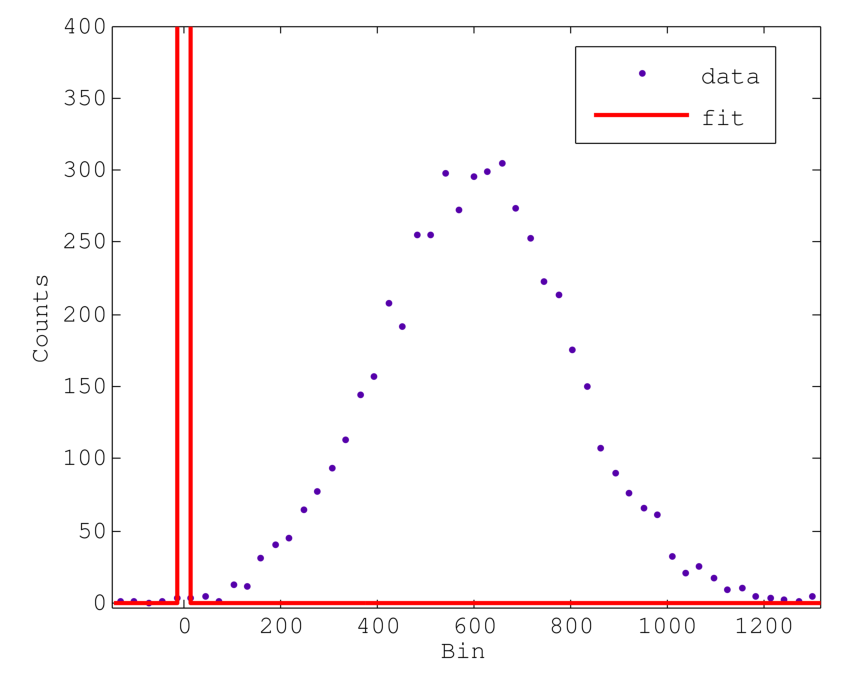
\includegraphics[scale=1]{gausnotwork.pdf}
 \caption{Fitting gaussian data generated on a computer with the function $ \mathtt{f(x)} =  \mathtt{a1}*\mathtt{exp}(-((\mathtt{x-b1})/\mathtt{c1})^\wedge \mathtt{ 2})$ in MATLAB. Choosing initial conditions of $\texttt{a1} = 1, \texttt{b1} = 0, \texttt{c1} = 1$, the computer algorithm that tries to minimize $\chi^2$ diverges.}
  \label{gausnotwork}
 \end{figure}
\end{center}
To fix this problem, and{ \it in general whenever you start any nonlinear fit}, it is a good idea to calculate a ballpark estimate of where the parameters should end up. In the example above, we know that the peak of the gaussian function should be about 300 high and located somewhere around 600 with a standard deviation on the order of 200. If we just start with parameters decently close to their final outcome, e.g. $\texttt{a1} = 300, \texttt{b1} = 600, \texttt{c1} = 200$, we get the following fit output:
\begin{framed}
\begin{verbatim}
General model Gauss1:
     f(x) =  a1*exp(-((x-b1)/c1)^2)
Coefficients (with 95% confidence bounds):
       a1 =   296.88732  (290.61741, 303.15724)
       b1 =   603.50693  (598.73503, 608.27883)
       c1 =   276.73864  (269.98996, 283.48732)

Goodness of fit:
  SSE: 3605
  R-square: 0.9934
  Adjusted R-square: 0.9931
  RMSE: 8.758
\end{verbatim}
\end{framed}
And the plot looks \emph{much} better:

\begin{center}
\Large \avantfont{ Good model with a good fit}

 \begin{figure}[H]
 
 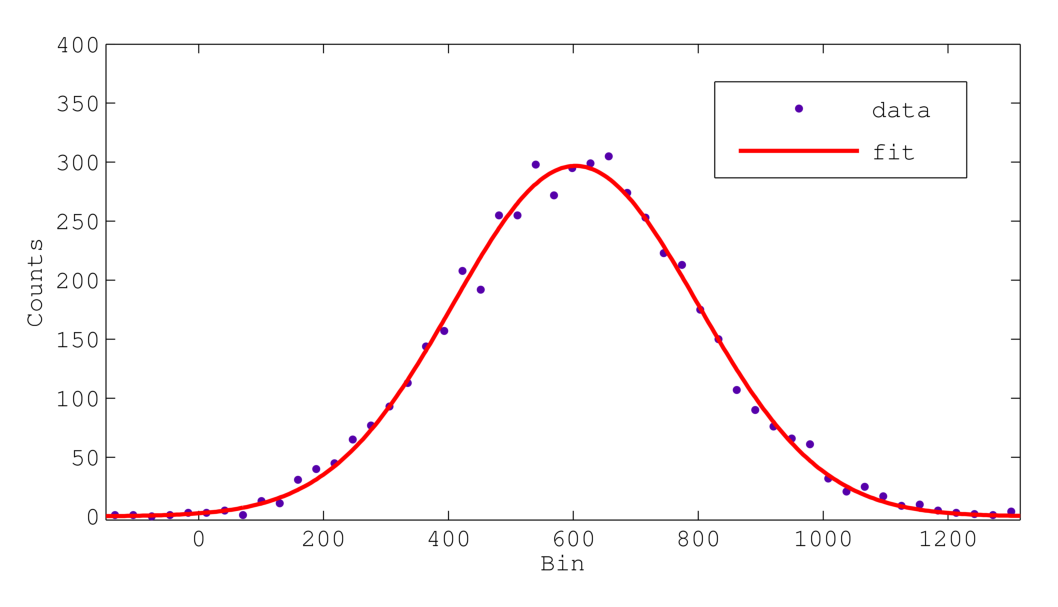
\includegraphics[scale=.9]{gauswork.pdf}
 \caption{Fitting gaussian data generated on a computer with the function $ \mathtt{f(x)} =  \mathtt{a1}*\mathtt{exp}(-((\mathtt{x-b1})/\mathtt{c1})^\wedge \mathtt{ 2})$ in MATLAB. Choosing initial conditions of $\texttt{a1} = 300, \texttt{b1} = 600, \texttt{c1} = 200$, the computer algorithm that tries to minimize $\chi^2$ settles to a good estimate.}
  \label{gauswork}
 \end{figure}
\end{center}
Now that we have a good fit, how can we use the fit output in a physics paper or report? The output that is produced is in the confidence interval format, which is a perfectly reasonable format to quote. For example, you could say:
\begin{framed}
``After fitting the data with a gaussian using a trust-region nonlinear least squares algorithm (default in MATLAB), we found the peak parameter $b$ converged to a value of 604 within a 95\% confidence interval (599, 608)."
\end{framed}
How do we decide what significant figures to use when the computer, when run long enough, could calculate 95\% confidence intervals out to 500 decimal places? It's not the lowest number of significant figures in the data, because the point of a fit is to reduce uncertainty by means of statistical analysis. The answer is that the confidence interval \texttt{(598.73503, 608.27883)}, as a measure of uncertainty, determines to what extent the parameter value \texttt{603.50693} is useful. The confidence interval can be expressed alternatively as \texttt{603.50693 (+ 5.7719, -  4.7719)}, at which point it becomes clear that everything after the ones' place is not useful (the uncertainty is of order 10$^0$. Now to get to an answer in the usual format of $\hat \mu \pm \hat \sigma$ must first convert to 68\% confidence (1$\sigma$) intervals by dividing the deviations by $1.96$. This is because a 95\% of a normal distribution lies between $-1.96\sigma$ and $+1.96\sigma$. So, enforcing significant figures, the value of \texttt{604 $\pm$ 5} at the 95\% confidence level becomes \texttt{604 $\pm$ 3}
at the standard 68\% confidence level.
\begin{framed}
{\bf In summary, if you are having problems with fitting, there are really only two things that can go wrong: either you're not looking for a minimized $\chi^2$ in the right place or you're using the wrong model.}
\end{framed}

\section{Evaluating Fits -- reduced $\chi^2$}
If you don't have the right model, how do you know in what way it's wrong? Well, there are really only two ways in which a model can be wrong.
\begin{enumerate}
\item {\bf The model oversimplifies the experiment.} When you haven't taken all of the physics into account, and your model at best only roughly approximates the data you've collected, there will likely be no combination of parameters that fit the data very well. 
\item {\bf The model overcomplicates the experiment.} When you have taken the physics of the experiment into account, and use extra parameters to describe the data, you will likely find a few combinations of parameters that work to describe the data very well. This means that the complexity of your model is {\it artificial} and does not reflect reality.
\end{enumerate}
To see whether the model is appropriate, physicists use a tool called reduced chi-squared ($\chi^2_{\text{red}}$). This is a quantity which represents the ratio of the estimated uncertainty in the model fit to the estimated uncertainty from experiment. Recall that $\chi^2$ was defined earlier as:
\begin{equation}
\chi^2= \sum_i \bigg (\frac{y_i - \hat y_i}{\hat \sigma_i} \bigg )^2
\end{equation}
Since $y_i - \hat y_i$ is the deviation of the data point $y_i$ from the model fit $\hat y_i$, and $\hat \sigma_i$ is the uncertainty calculated for the experiment at that data point, the contribution of any datapoint to $\chi^2$ is near one when the deviation of the model is about the same size as the uncertainty. What this means is that if we divide $\chi^2$ by the number of datapoints and get something close to one, then we can say that our model is good so long as we are confident in our estimate of uncertainty. Just like with Bessel's correction of the estimated standard deviation however (eq. \ref{bessel} ), we can't simply divide by the number of data points we have -- we have to divide by the \emph{degrees of freedom} $\nu = N - k - 1$.
\begin{equation}
\chi^2_{\text{red}} =   \frac{1}{\nu} \sum_i \bigg (\frac{y_i - \hat y_i}{\hat \sigma_i} \bigg )^2 = \frac{\chi^2 }{\nu}
\end{equation}
 As before, $N$ is the number of data points and $k$ is the number of parameters in the model. Of course, if $k+1 \ll N$, then this correction doesn't make much difference (it is however formally correct). When we accept $\chi^2_{\text{red}}$ as a good estimate of the ratio of model deviation to expected deviation, we can evaluate whether the model is good by examining the following cases:
 \begin{framed}
 \begin{easylist}[enumerate]
 & $\chi^2_\text{red} \gg 1$ . When the reduced chi-squared of a fit is much larger than one, the only possible ways for this to happen are for:
 && the model to fit so poorly that $(y_i - \hat y_i)^2 \gg (\hat \sigma_i)^2$ on average.
 && the uncertainty $ \hat \sigma_i$ to be so underestimated that $(y_i - \hat y_i)^2 \gg (\hat \sigma_i)^2$ on average, \emph{even though} the model fits fairly well. This is only practically possible if you think you have much more precision on your individual measurements than you \emph{actually} do. 
 & $\chi^2_\text{red} < 1$. When the reduced chi-squared of a model fit is less than one, the only way for this to happen is for the error in your fit to be overestimated so that $(y_i - \hat y_i)^2 < (\hat \sigma_i)^2$  on average. 
 \end{easylist}
 \end{framed}







% BAD STARTING POINTS
%General model Gauss1:
%     f(x) =  a1*exp(-((x-b1)/c1)^2)
%Coefficients (with 95% confidence bounds):
%       a1 =   100.00000
%       b1 =     1.00000
%       c1 =     0.00000
%
%Goodness of fit:
%  SSE: 1.048e+06
%  R-square: -0.913
%  Adjusted R-square: -0.9944
%  RMSE: 149.3
%
%  Warning: A negative R-square is possible if the model
%           does not contain a constant term and the fit
%           is poor (worse than just fitting the mean).
%           Try changing the model or using a different StartPoint.
% GOOD STARTING POINTS
%General model Gauss1:
%     f(x) =  a1*exp(-((x-b1)/c1)^2)
%Coefficients (with 95% confidence bounds):
%       a1 =   296.88721  (290.61729, 303.15712)
%       b1 =   603.50687  (598.73496, 608.27877)
%       c1 =   276.73886  (269.99018, 283.48755)
%
%Goodness of fit:
%  SSE: 3605
%  R-square: 0.9934
%  Adjusted R-square: 0.9931
%  RMSE: 8.758
%
%\subsection{Drosg's Seven Myths in Error Analysis}
%
%
%\begin{enumerate}
%\item Random errors can always be determined by repeating measurements under identical conditions.
%\item Systematic errors can be determined inductively
%\item Measuring is the cause of all errors
%\item Counting can be done without error
%\item Accuracy is more important than precision
%\item It is possible to determine the sign of an error
%\item It is all right to ``guess'' an error
%\end{enumerate}
